\begin{flushright}{\kaishu 天\ 工\ 开\ 物\ !\\「Made in Heaven!」要开始加速了\footnote{ジョジョの奇妙な冒险 Part 6
  スト-ンオ-シャン}}\end{flushright}

\section{极限和连续性}\label{011}

跳过一些内容: 集合 (set), 点集拓扑 (point set topology), 数列与级数
(sequence and series); 如果您希望习得更加严谨的数学语言, 那么可以移步
Walter Rudin - \emph{Principles of Mathematical Analysis} (俗称 baby
Rudin\footnote{Baby = 数学分析原理 \emph{Principles of Mathematical
  Analysis}; Papa/Big = 实分析与复分析 \emph{Real and Complex Analysis};
  Grandpa = 泛函分析 \emph{Functional Analysis}; 好好地学严格的数学,
  逃不掉这三本分析, 这个系列也就看个乐子.}).

\subsection{极限 (limit)}

\begin{tcolorbox}[size=fbox, breakable, enhanced jigsaw, title={定义}]
当 $x$ 趋向于 $p$ 时, $x\rightarrow p$ , $f(x)$
趋向于 $q$, $f(x)\rightarrow q$ , 记作
$\lim_{x\rightarrow p}f(x)=q.$

用 $\epsilon - \delta$ 语言 (出现了!) 来说,
$\lim_{x\rightarrow p}f(x)=q$ 便是: 对于任意的 $\epsilon>0$ , 存在
$\delta>0$ 使得【若 $0<|x-p|<\delta$, 便有 $|f(x)-q|<\epsilon$
】\footnote{其实这里的定义还是很不严谨, 比如没有说明定义域和值域.
  为了省笔墨下文都默认取值范围在合适的区间内.}.

\end{tcolorbox}

为什么要用 $\epsilon - \delta$ 语言? 原本的``趋向于''其实很不严格,
什么叫趋向于呢, 于是 $\epsilon - \delta$ 语言如是说道:

\begin{itemize}

\item
  我先任意选定一个 $\epsilon$,
\item
  然后我要试着找到一个 $\delta$,
\item
  使得 $x$ 与 $p$ 足够接近时 - 有多接近呢? 它们差的绝对值
  (或者说``距离'', 不过这边还没定义距离, 233) 小于 $\delta$ - 便有
  $f(x)$ 与 $q$ 足够接近 - 多近呢? 他们差的绝对值小于 $\epsilon$.
\item
  若对于任意小的 $\epsilon$, 总能找到一个这样的 $\delta$,
  那么便可以放心地说, 确有$\lim_{x\rightarrow p}f(x)=q$.
\end{itemize}

\begin{tcolorbox}[size=fbox, breakable, enhanced jigsaw]
  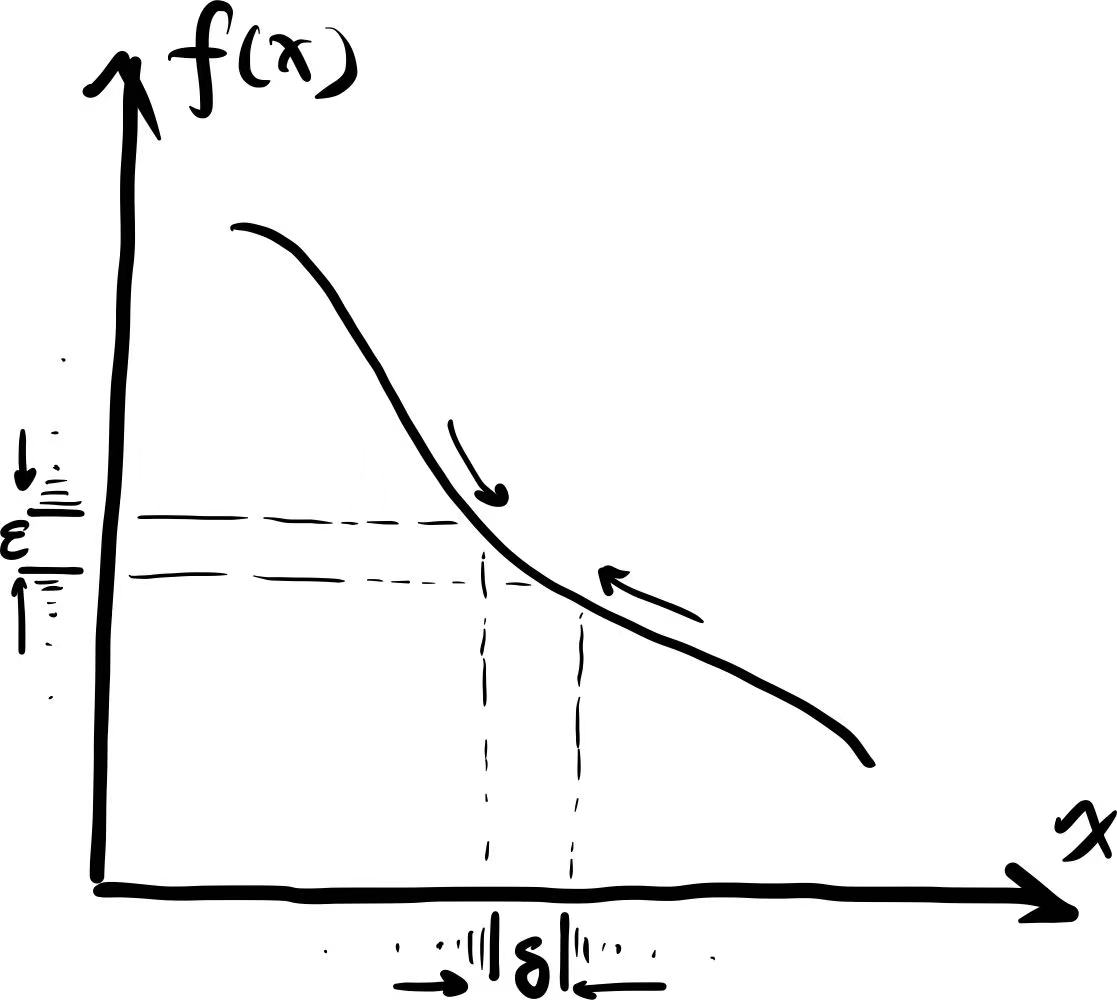
\includegraphics[width=0.45\textwidth]{img/image-20230503152041842.png}
\end{tcolorbox}

\begin{newquote}
\textbf{例子}: 一个平凡的情况 (a trivial case), $f(x)=ax$, 证明
$\lim_{x\rightarrow 1}f(x)=a$.

\textbf{思路} (草稿纸上或者脑子里的部分): 对于任意 $\epsilon>0$
我们需要找到 $\delta>0$, 满足当 $0<|x-1|<\delta$ 时,
$|f(x)-a|<\epsilon$ 成立.

\begin{itemize}
\item
  $|f(x)-a|=|ax-a|=a|x-1|$
\item
  令上式小于 $\epsilon$, 发现有 $|x-1|<\epsilon/a$
\item
  令 $\delta=\epsilon/a$ , 即可出锅食用 (bushi).
\end{itemize}

\textbf{证明} (写下来的正式的书面的部分): 对任意 $\epsilon>0$ , 令
$\delta=\epsilon/a$, 则当 $0<|x-1|<\delta$ 时, 有

\begin{itemize}

\item
  $|f(x)-a|=|ax-a|=a|x-1|<a\delta<\epsilon$.
\item
  于是根据极限的定义, $\lim_{x\rightarrow 1}f(x)=a$
\end{itemize}

Q.E.D\footnote{Quod erat demonstrandum - 这被证明了.}

\textbf{吐槽}: 鄙人学分析的时候学得就很不到位,
写证明的时候常常向同学``借鉴'', 时常觉得, 证明本身并不难写,
难得是想到并``构造''出一些证明需要的东西, 就如在上面的例子中构造一个
$\delta=\epsilon/a$;
殊不知``借鉴''的那些作业其实只有上面例子中【证明】的部分,
而【思路】部分被写在草稿纸上丢掉了.
这种狡猾如雪地上的狐狸一般用尾巴扫去自己的踪迹的行为\ldots{}
于是有这样的说法:

一位菲尔兹得主告诉我, 顶级的数学家们会秘密地像物理学家一样思考,
等他们得到证明的一个大框架之后, 他们再用 epsilon 和 delta
的语言把证明过程包装起来.
\end{newquote}

\begin{itemize}

\item
  若 $f(x)$ 在 $x\rightarrow p$ 处存在极限,
  这个极限是\textbf{唯一}的 (unique).
\end{itemize}

考虑 $\lim_{x\rightarrow p}f(x)=a$, $\lim_{x\rightarrow p}g(x)=b$,
极限还存在以下规律 (啊, 美好的线性) :

\begin{itemize}

\item
  $\lim_{x\rightarrow p}(f\pm g)(x)=a\pm b$;
\item
  $\lim_{x\rightarrow p}(fg)(x)=ab$;
\item
  $\lim_{x\rightarrow p}\frac{f}{g}(x)=\frac{a}{b}$, 若 $b\neq 0$.
\end{itemize}

\begin{newquote}
回收一个坑. 【\ref{002}\nameref{002}】中提到过 $\mathrm{0}^0$ 是未被定义的问题,
一种解释便是, 若希望用极限来定义它的取值, 那么应该从
$\lim_{x\rightarrow0}x^0$ 出发, 得到 $1$, 还是应该从
$\lim_{x\rightarrow0}0^x$ 出发, 得到 $0$?
\end{newquote}


\subsection{连续性 (continuity)}

\textbf{定义}: 对于一函数 $f(x)$, 对于任意的 $\epsilon>0$ , 存在
$\delta>0$ 使得【对于某个特定的 $x_0$, 若有 $x$ 满足
$|x-x_0|<\delta$, 便有 $|f(x)-f(x_0)|<\epsilon$】, 那么我们便可以说,
$f(x)$ 在 $x_0$ 处连续.

\begin{itemize}

\item
  若 $f(x)$ 和 $g(x)$ 连续, 那么 $f(g(x))$ 也连续.
\item
  若 $f(x)$ 和 $g(x)$ 连续, 那么 $(f\pm g)(x)$, $fg(x)$,
  $\frac{f}{g}(x)$ 都连续, 最后一条要求 $g(x)$ 对于任意 $x$ 不为
  $0$.
\end{itemize}

从连续性出发, 可以得到以下几个定理, 图像上非常直观, 这边暂时忽略严格证明.

\begin{tcolorbox}[size=fbox, breakable, enhanced jigsaw, title={极值定理 (extreme value theorem)}]

\begin{tcolorbox}[size=fbox, breakable, enhanced jigsaw, sidebyside]
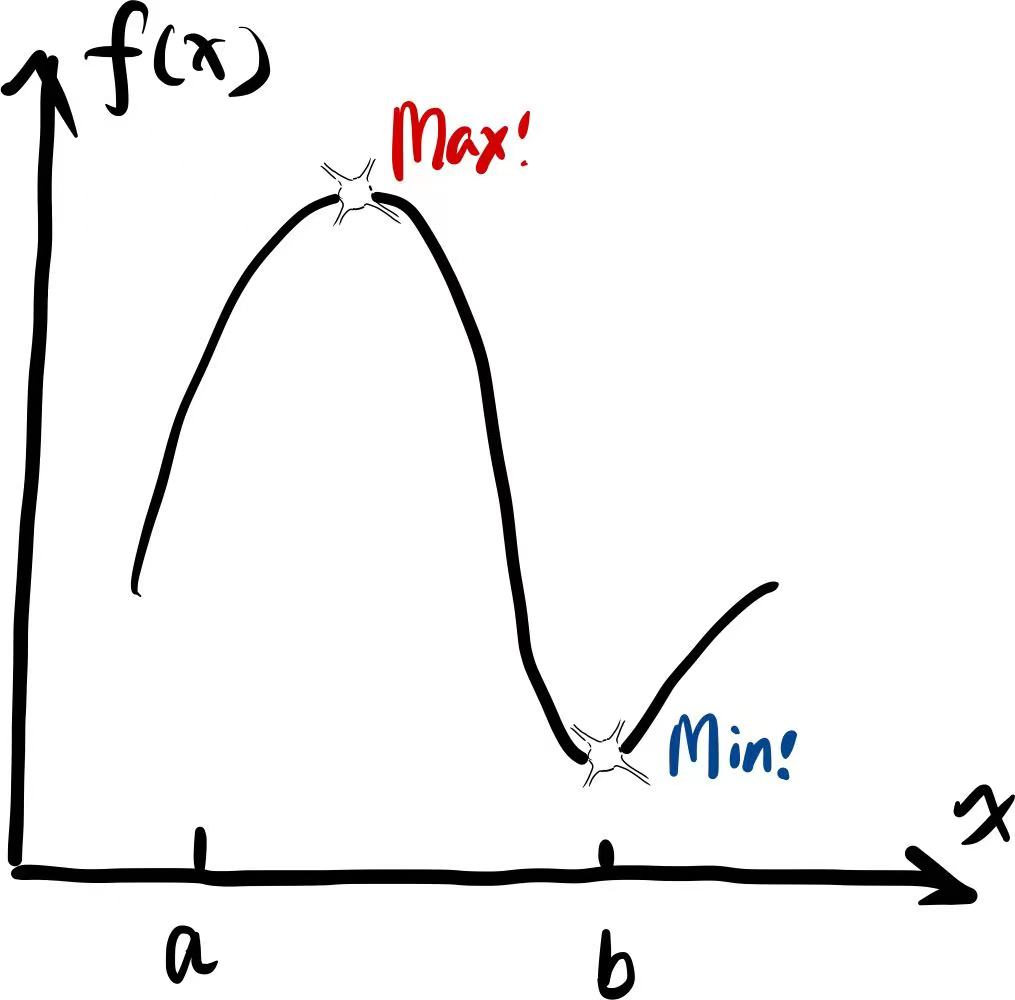
\includegraphics[width=0.9\textwidth]{img/image-20230503152124313.png}
\tcblower
\kaishu{\small 若函数 $f(x)$ 在区间 $[a,b]$ 连续, 则 $f(x)$ 必然在区间 $[a,b]$
存在最大值和最小值.}
\end{tcolorbox}

\end{tcolorbox}

\begin{tcolorbox}[size=fbox, breakable, enhanced jigsaw, title={介值定理 (intermediate value theorem)}]

\begin{tcolorbox}[size=fbox, breakable, enhanced jigsaw, sidebyside]
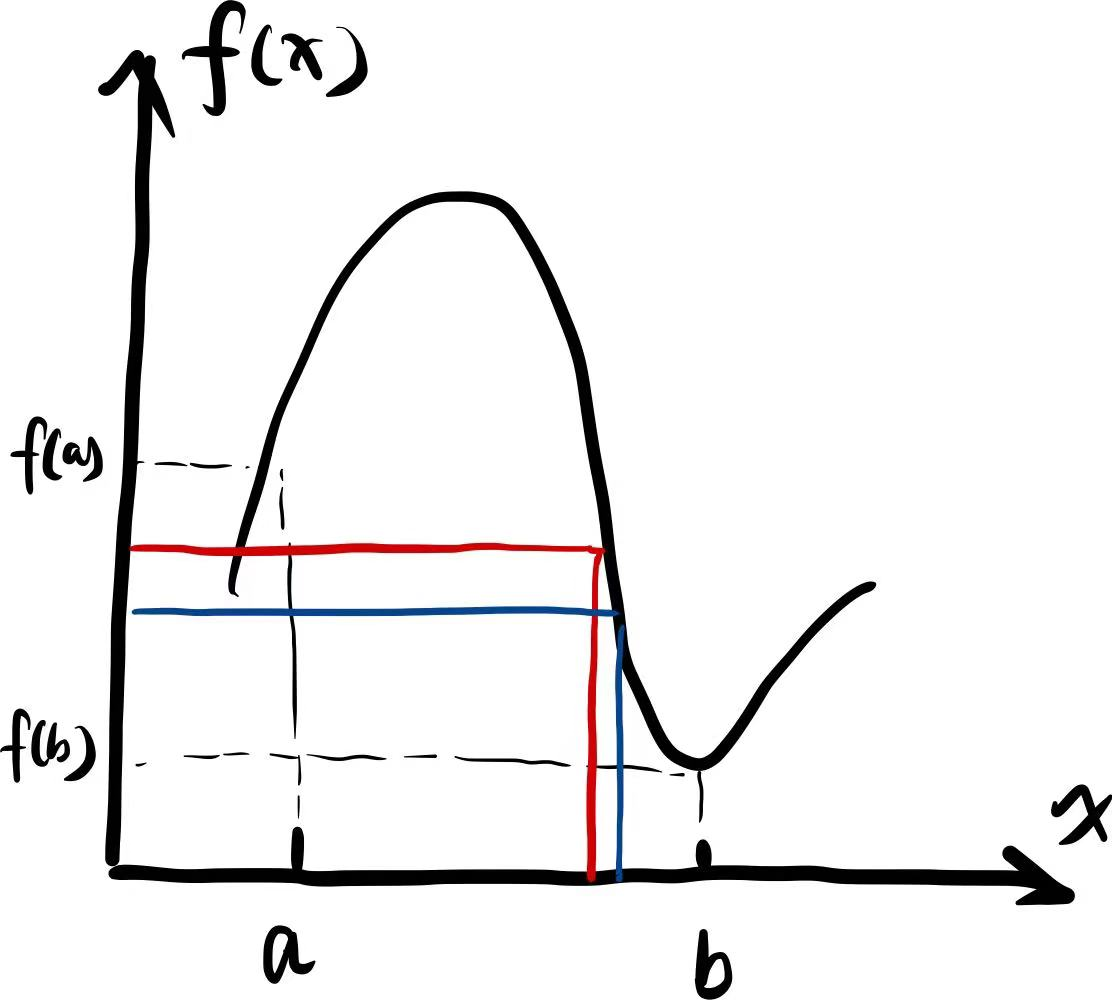
\includegraphics[width=0.9\textwidth]{img/image-20230503152147199.png}
\tcblower
\kaishu{\small 若函数 $f(x)$ 在区间 $[a,b]$ 连续, 且有 $f(a)<C<f(b)$ 或
$f(a)>C>f(b)$, 那么总是存在 $c\in(a,b)$ 或者说 $a\le c\le b$ 使得
$f(c)=C$.}
\end{tcolorbox}

\end{tcolorbox}

\begin{tcolorbox}[size=fbox, breakable, enhanced jigsaw, title={零点定理 (zero theorem)}]

\begin{tcolorbox}[size=fbox, breakable, enhanced jigsaw, sidebyside]
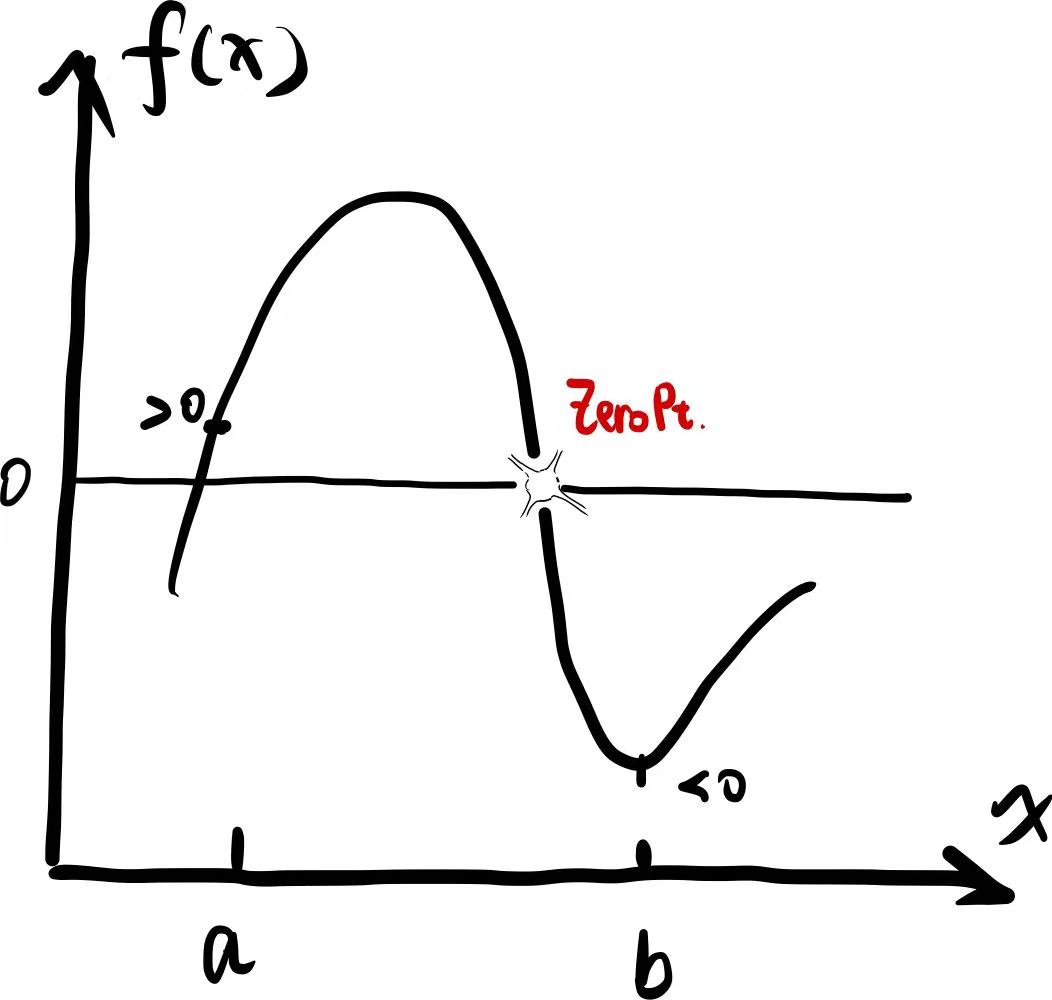
\includegraphics[width=0.9\textwidth]{img/image-20230503152707849.png}
\tcblower
\kaishu{\small 若函数 $f(x)$ 在区间 $[a,b]$ 连续, 且$f(a)f(b)<0$, 则存在
$c\in(a,b)$ 使得 $f(c)=0$.}
\end{tcolorbox}

\end{tcolorbox}
